\chapter{Design}~\label{cha:design}

Before initiating detailed design work, it was decided this project would be a web application accessible via a browser. This approach offers several advantages, such as cross-platform compatibility, ease of access (requiring only a browser), scalability, and the ability to leverage existing web technologies~\cite{6822300}. With this established, a plan was formulated, encompassing architectural decisions, technology stack selection, and the definition of testing criteria.

\section{Architecture}
The system architecture defines the overall structure of the project and the communication between its components. For this project, two architectural approaches were considered: a monolithic architecture and a microservices-based architecture.

\subsection{Monolithic}
For this project, the monolithic approach offers several benefits. With all code centralized within a single framework, development is simplified, and debugging becomes more straightforward. Additionally, initial deployment is less complex since only one program needs to be managed once development is complete~\cite{9109514}.

However, the monolithic design has its drawbacks. As the system grows, maintaining a large, integrated codebase can become increasingly challenging; test suites may grow more complex and time-consuming to execute. During deployment, a single fault could potentially bring down the entire system, resulting in a complete loss of service. Similarly, even minor updates would require redeploying the entire monolith, increasing the risk of downtime. Moreover, this approach does not scale as effectively for web applications; as user demand increases, the need to redeploy the monolith frequently to manage higher request volumes becomes a significant concern~\cite{9109514}.

Although the scope of this project is small and so the drawbacks of a monolithic approach would have minimal impact, it was determined that the project should be designed to be fully scalable. With the potential for future growth in features and user base, the limitations inherent in a monolithic architecture would eventually become a hindrance in this scenario. Consequently, the monolithic approach was ruled out in favour of a more scalable architectural model.

\begin{figure} [H]
    \centering
    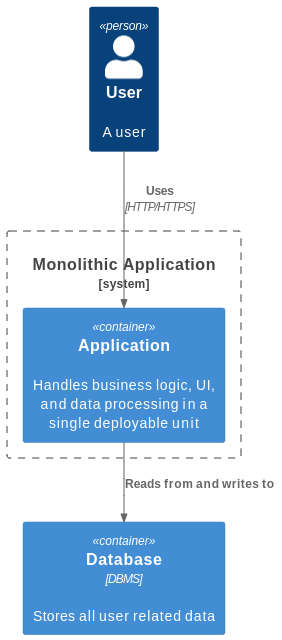
\includegraphics[width=0.35\linewidth]{figures/monolithic_arch.png}
    \caption{A potential architecture for a monolithic approach}
~\label{fig:monolith-arch}
\end{figure}

\subsection{Microservices}
The alternative approach examined was the use of microservices. In this architecture, the application's functionality is divided into separate services that communicate with each other using standardized protocols such as HTTP.\@

The primary benefits of this approach pertain to deployment and maintenance. Once deployed, the system can be scaled more efficiently—only those services experiencing high demand need to be replicated, which is significantly faster and more resource-efficient than scaling a monolithic system. Additionally, maintenance is simplified because each service operates independently; developers can focus on individual components without needing a comprehensive understanding of the entire system something that can become difficult even in small systems like this project.

However, the increased complexity of managing multiple services means that initial deployment is more challenging. Configuring the different addresses for inter-service communication can prove to be difficult, and each service requires setup that would only need to be completed once for a monolith. Nonetheless, once this initial configuration is completed, development within a microservices architecture becomes as straightforward as working with a monolithic architecture.

\begin{figure} [H]
    \centering
    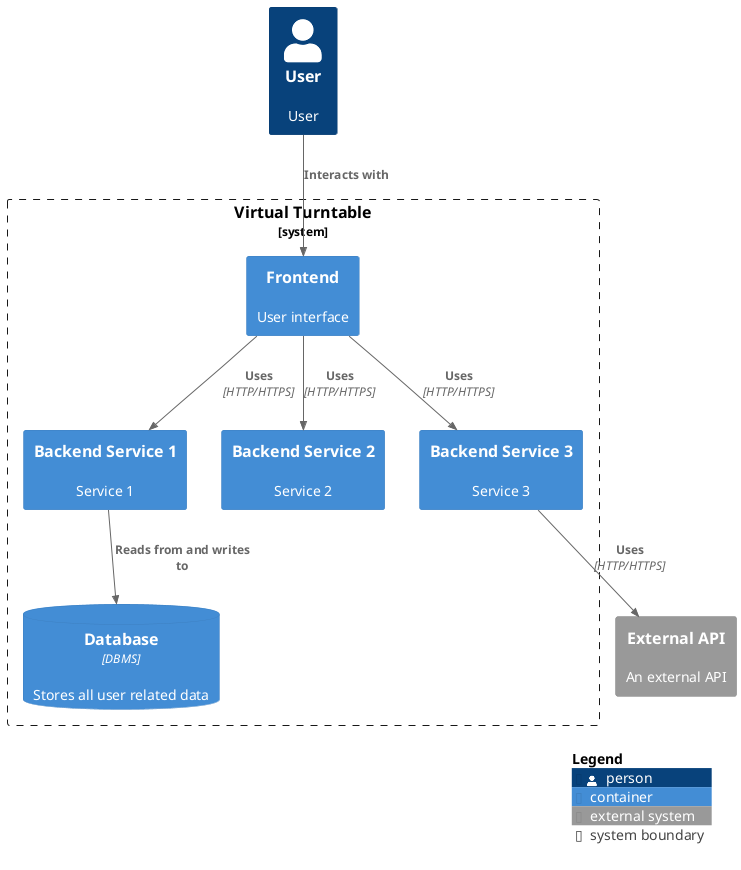
\includegraphics[width=0.5\linewidth]{figures/microservices_arch.png}
    \caption{A potential microservices design with three backend services}
    \label{fig:microservices-arch}
\end{figure}

\subsection{Final design}
The final design employs a microservices approach alongside a backend-for-frontend (BFF) design pattern. In this pattern, a dedicated backend service is created for each type of frontend application, such as desktop or mobile, ensuring that each backend caters specifically to a specific interface’s requirements. This pattern leverages the benefits of a microservices architecture and helps to maintain complexity by isolating functionality~\cite{BFF}. Details about each microservice are described in Section~\ref{sec:backend-design}.

\begin{figure} [H]
    \centering
    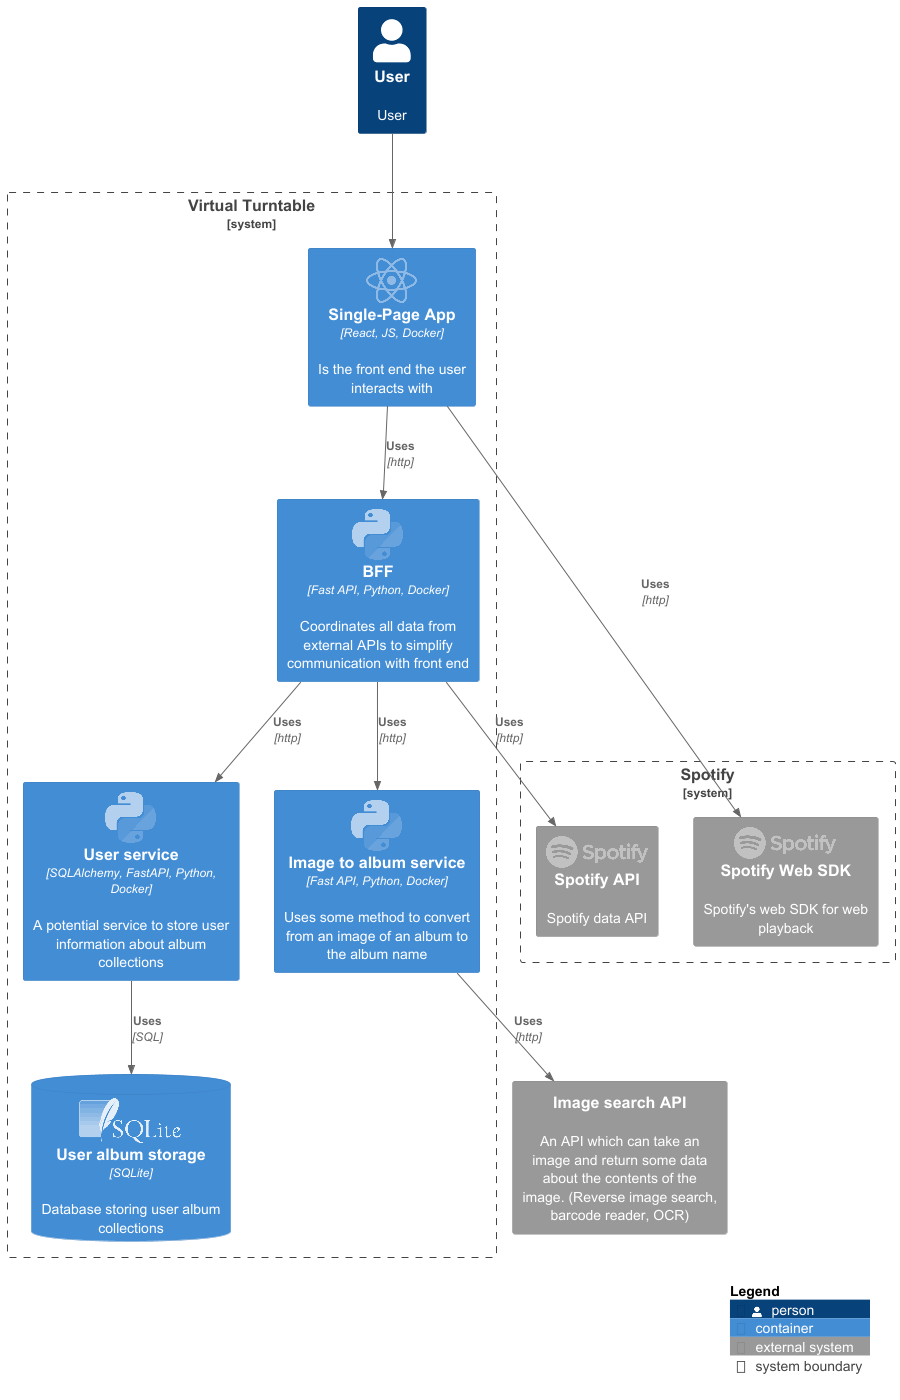
\includegraphics[width=0.5\linewidth]{figures/final_arch.png}
    \caption{The final architecture including technologies and external APIs}
    \label{fig:final-arch}
\end{figure}


\section{Technologies}
\subsection{FastAPI}
FastAPI is a Python web framework for building APIs, offering automatic input validation via Pydantic and seamless relational database integration with SQLAlchemy~\cite{FastAPI}. Compared to other popular frameworks like Django and Flask, FastAPI was particularly well-suited for this project due to its lightweight nature and built-in compatibility with these technologies. This combination provided an optimal balance between ease of setup and feature-rich functionality.

FastAPI was extensively utilized to develop all backend services in this project. Its straightforward setup allowed for rapid initial development, enabling quick implementation of basic functionality.

The backend primarily operated through individual API endpoints, which the frontend called to retrieve data as needed. Additionally, WebSockets facilitated asynchronous server-to-client communication, ensuring users were promptly notified of backend events, such as collections being shared with them.

\subsection{React}
React is a JavaScript library for building interactive web interfaces~\cite{React}. Its modular, component-based architecture was particularly beneficial in this project, enabling component reuse across multiple pages and reducing code duplication. A key advantage of this approach is the availability of extensive component libraries that provide pre-built functionality and styling for low-level elements, such as buttons. This allowed development efforts to focus on the application's bespoke features.

For this project, the HeroUI component library was utilized, offering a set of pre-designed components that were assembled into larger, more complex UI elements to create the final application.

React also managed the application's state and handled backend requests as needed. This enabled backend services to remain stateless, reducing complexity and improving scalability.

\subsection{Docker}
Docker is a platform for containerising applications, allowing them to run in isolated environments while communicating through specified exposed ports. This approach is a standard practice in modern web development and is widely supported by cloud providers, simplifying deployment and providing a consistent environment across different platforms.

For this project, Docker enabled fast and efficient deployment. Cloud providers could autonomously build and run the application when supplied with the codebase and Dockerfile. Additionally, for development, the containerised system could be easily executed on any device running Docker, eliminating the need for manual environment configuration.

All backend services and frontend, were containerised using Dockerfiles and deployed to a cloud provider, ensuring a scalable and reproducible deployment process.

\subsection{Spotify API And Web Playback}
The music service Spotify offers a suite of APIs for music-related services, including search and playback functionalities that matched the core features of this project. Given the impracticality of maintaining an independent album database, offloading the responsibility of maintaining a library of albums and music to Spotify was a logical choice.

Specifically, the search API was used to identify albums, while the playback API enabled streaming of the selected content.

However, a key limitation of this approach is that the playback API requires a Spotify Premium subscription. Though, as the Spotify API mandates user authentication via a Spotify account, this requirement allows the Spotify account to serve as the user account for the application, thereby reducing security concerns related to the storage and management of user data.

\subsection{Reverse Image Search}
Reverse image search is a form of content-based image retrieval that uses an image as the query to retrieve related results. This process involves extracting feature vectors, using algorithms such as SIFT, and comparing these against a collection of previously indexed images to return the closest matches~\cite{Gaillard2017LargeSR}.

In this project, reverse image search functionality was implemented to identify albums from images uploaded by users. Recognizing that maintaining an up-to-date, in-house database of album covers would be impractical, it was decided early on to leverage an external API.\@ Two reverse image search APIs were evaluated: Google and Bing. Although Bing's API was simpler to integrate, it frequently failed to accurately identify albums—even from images that were already indexed by Bing's image search. In contrast, Google's API demonstrated a much higher reliability in album identification. Given the critical importance of accurate album retrieval for the project, the Google API was ultimately chosen.

Compared to other methods for recognizing albums from images, such as optical character recognition (OCR) or barcode scanning, reverse image search was selected for its robustness. OCR can be unreliable when album covers feature stylised text or lack text entirely and barcode scanning, though dependable, requires a barcode to be present. This requirement is problematic, particularly since vinyl records may predate the widespread use of barcodes.

\subsection{Google Cloud}
Google Cloud is a collection of cloud services offered by google that can be used on a pay as you use basis. For this project two of their services were used: their reverse image search api and Google Cloud Run which was used to host the applications running in Docker containers.

TODO: Add detail about google cloud hosting















\section{Frontend}
This section details the design of the user interface.
\subsection{Principles}
The development of the user interface mainly involved sticking to a set of principles such as Shneiderman's eight golden rules of interface design \cite{Shneiderman}.

TODO: Add references to UI papers talking about web design principles
\subsection{Wireframe mockups}
Before beginning development for each page a wireframe mockup was made. These were low fidelity prototypes to be put together

\subsubsection{Play Screen}
Figure~\ref{fig:play_screen_mockup} shows the play screen mockup where the user will be playing their music. So it required controls that would be used to control playback including buttons to play, pause, skip to the next track, go back to the previous track, track position, and volume control. Along with this the intention to keep the feeling of a turntable the idea of scrubbing through the whole album rather than individual songs appears in the mockup.
\begin{figure} [H]
    \centering
    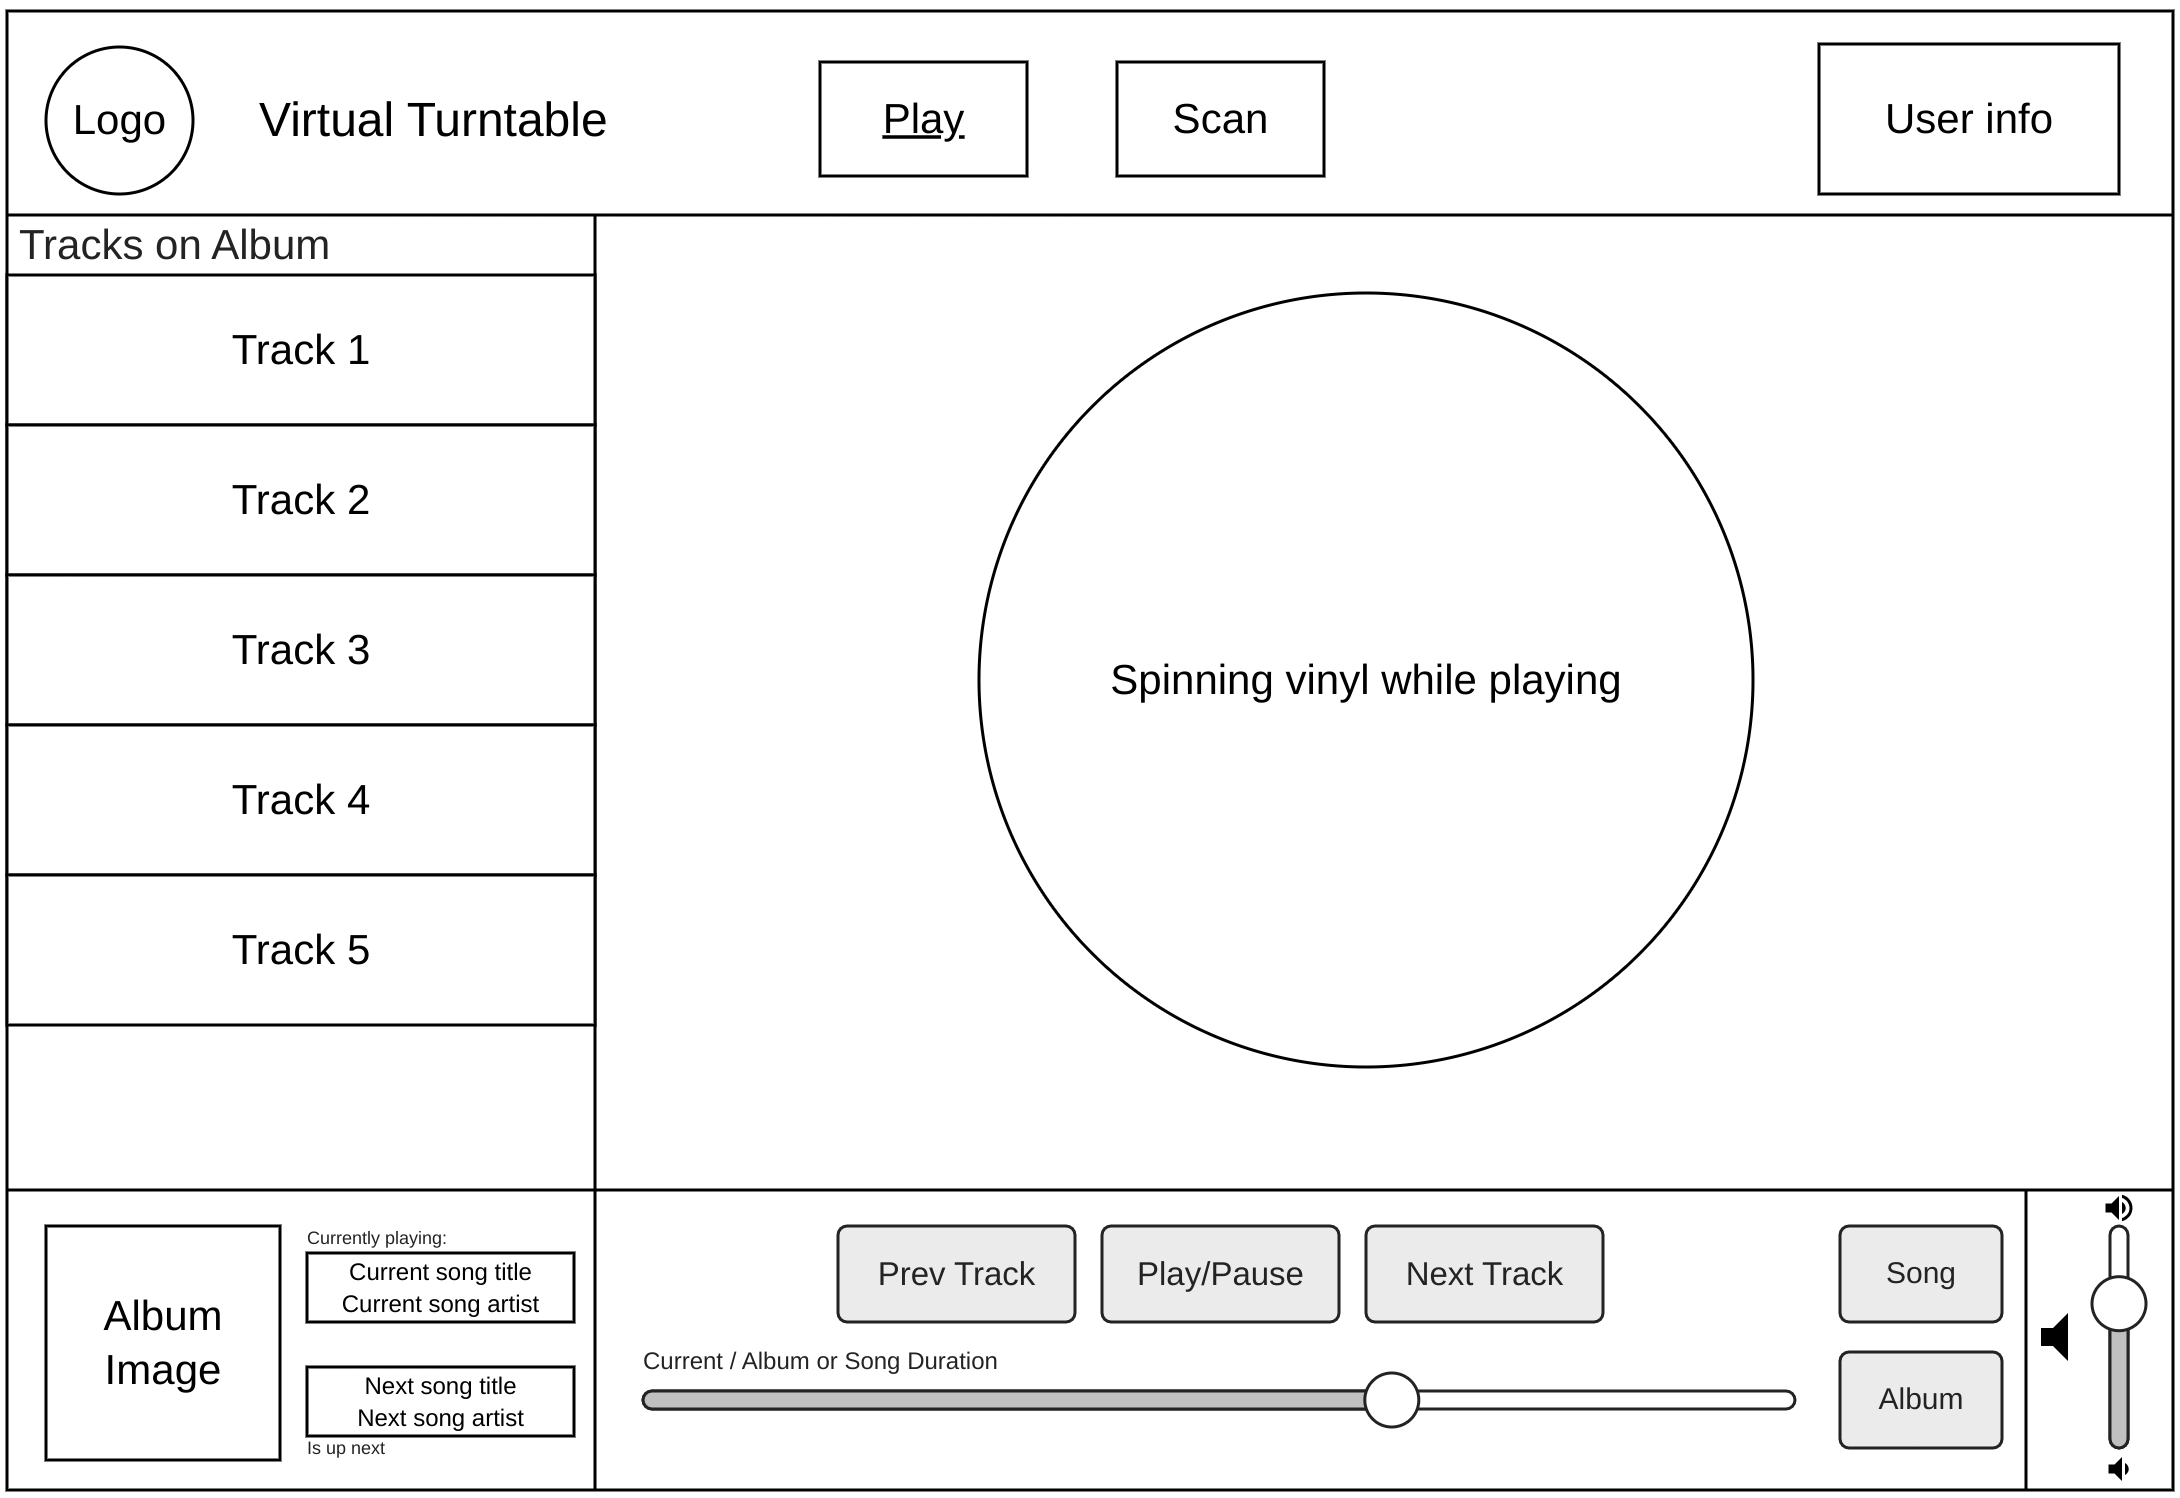
\includegraphics[width=0.6\linewidth]{figures/play_screen_mockup.png}
    \caption{The play screen wireframe mockup}
    \label{fig:play_screen_mockup}
\end{figure}

\subsubsection{Scanning Screen}
Figure~\ref{fig:scan_screen_mockup} shows the screen users would use to take a picture of or upload an image of their album to the application.
\begin{figure} [H]
    \centering
    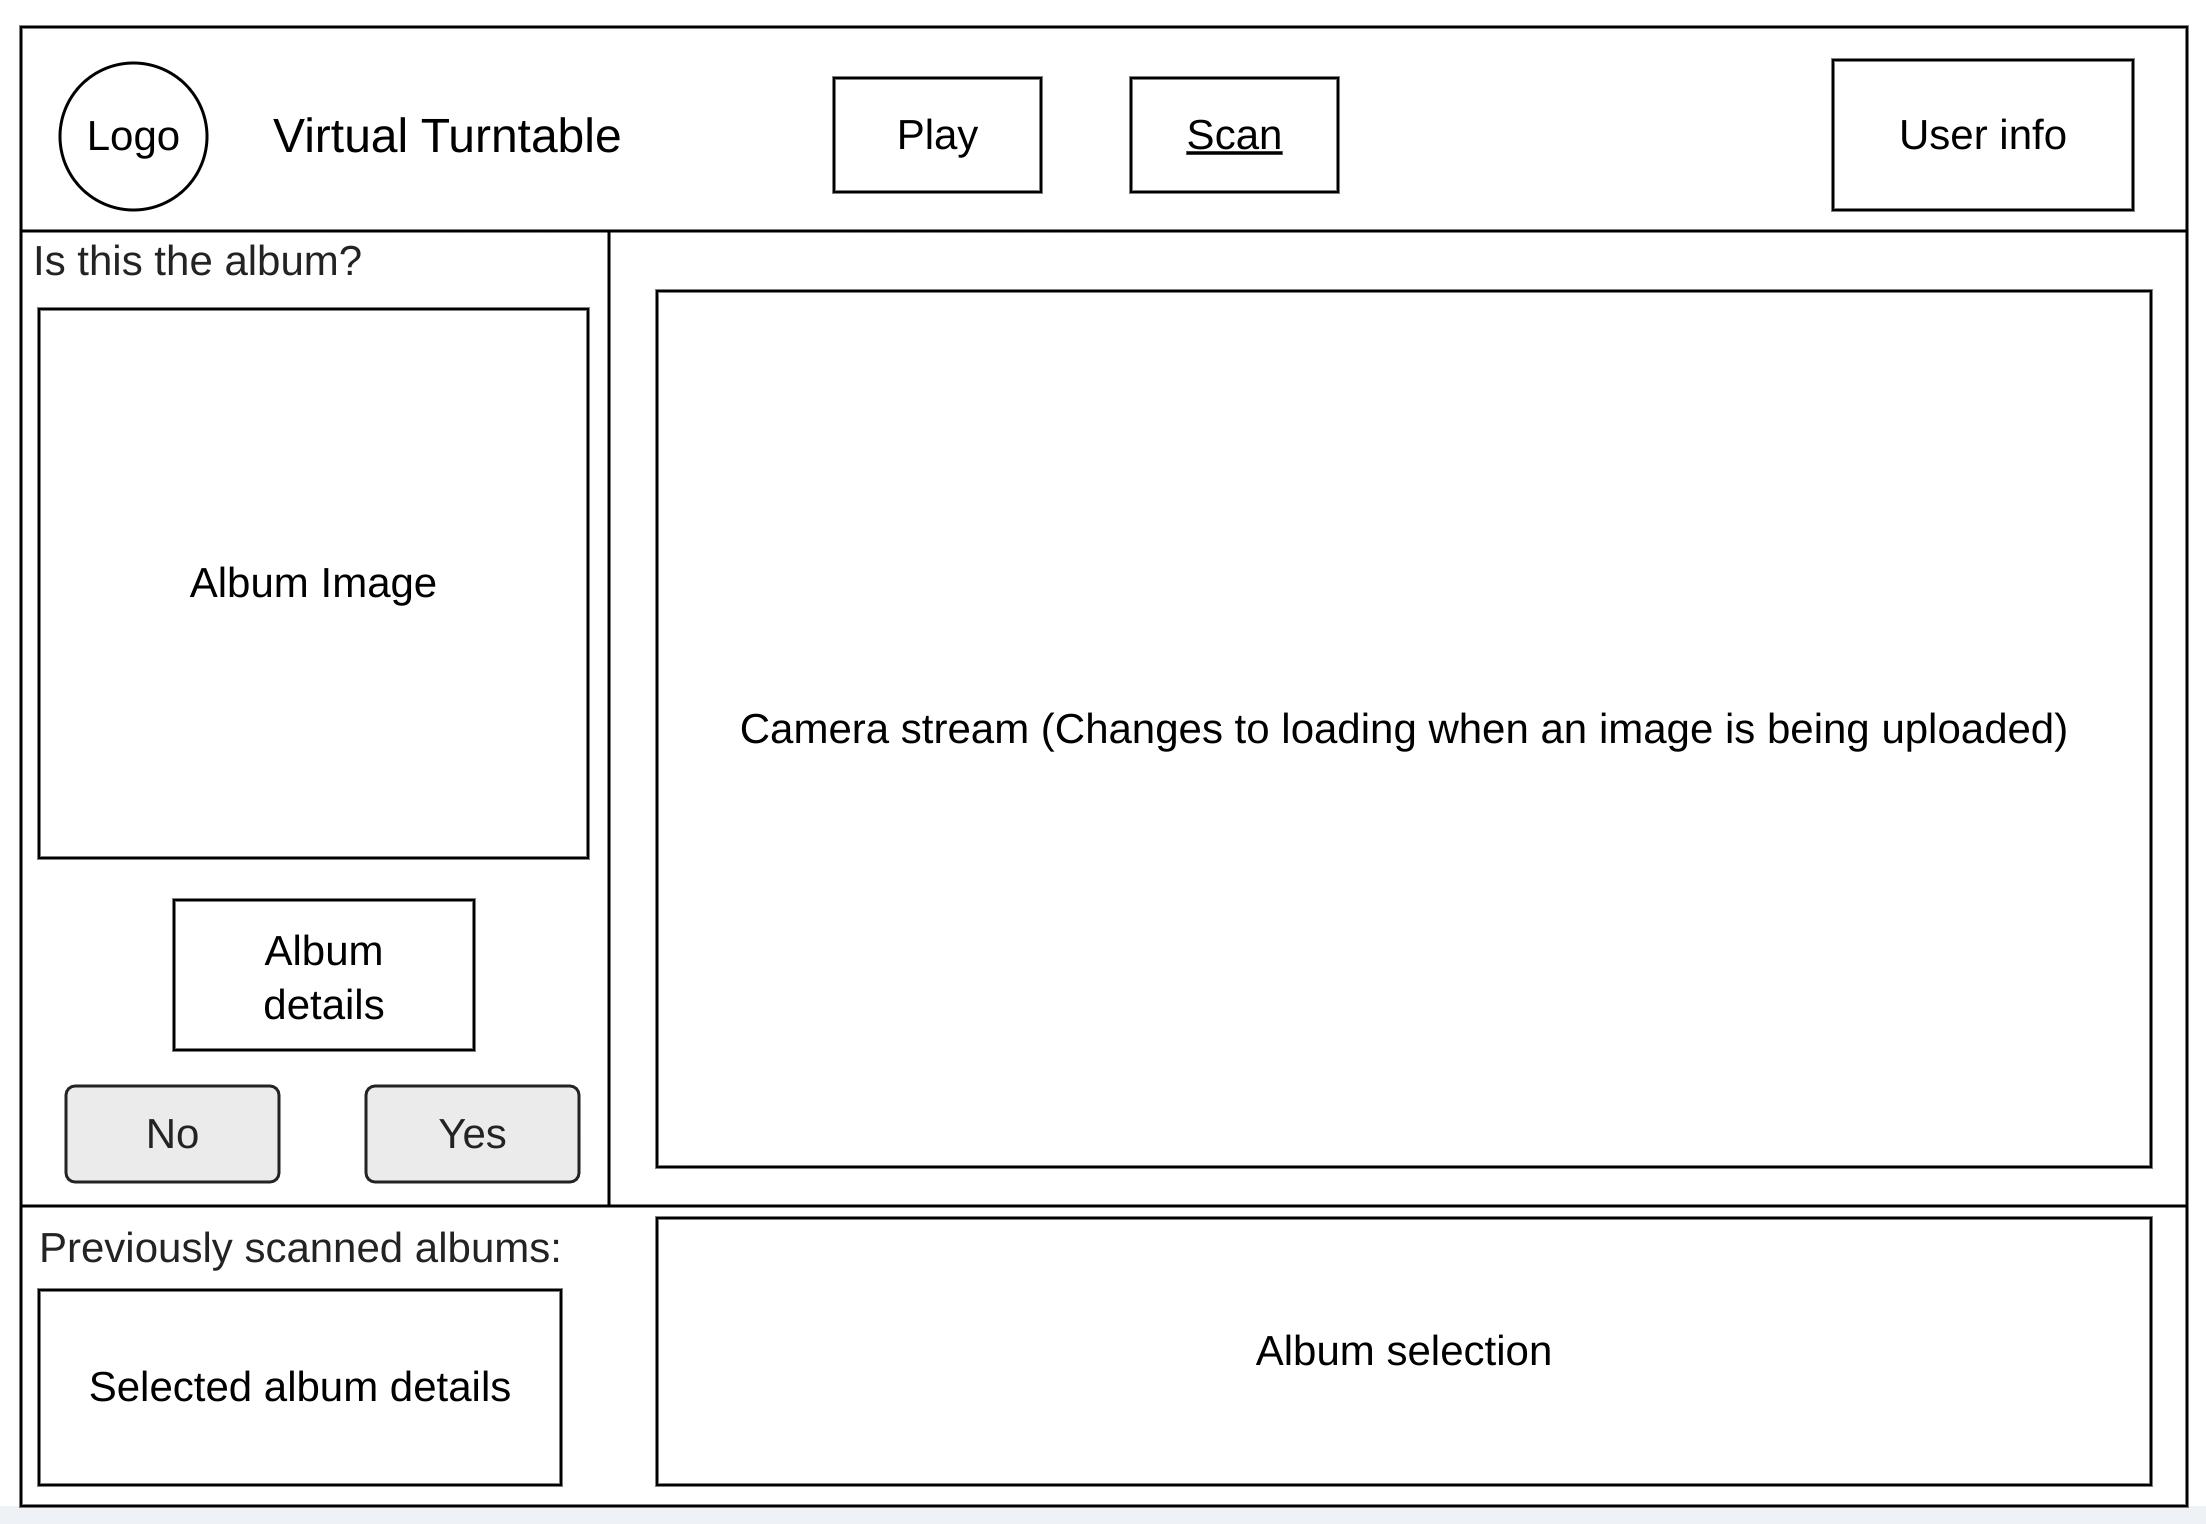
\includegraphics[width=0.6\linewidth]{figures/scan_screen_mockup.png}
    \caption{The scanning screen wireframe mockup}
    \label{fig:scan_screen_mockup}
\end{figure}


\subsubsection{Social Screen}
Figure~\ref{fig:social_screen_mockup} shows the social screen, a place to view other users collections stored on by the application including those shared directly with the user and those people have shared publicly.
\begin{figure} [H]
    \centering
    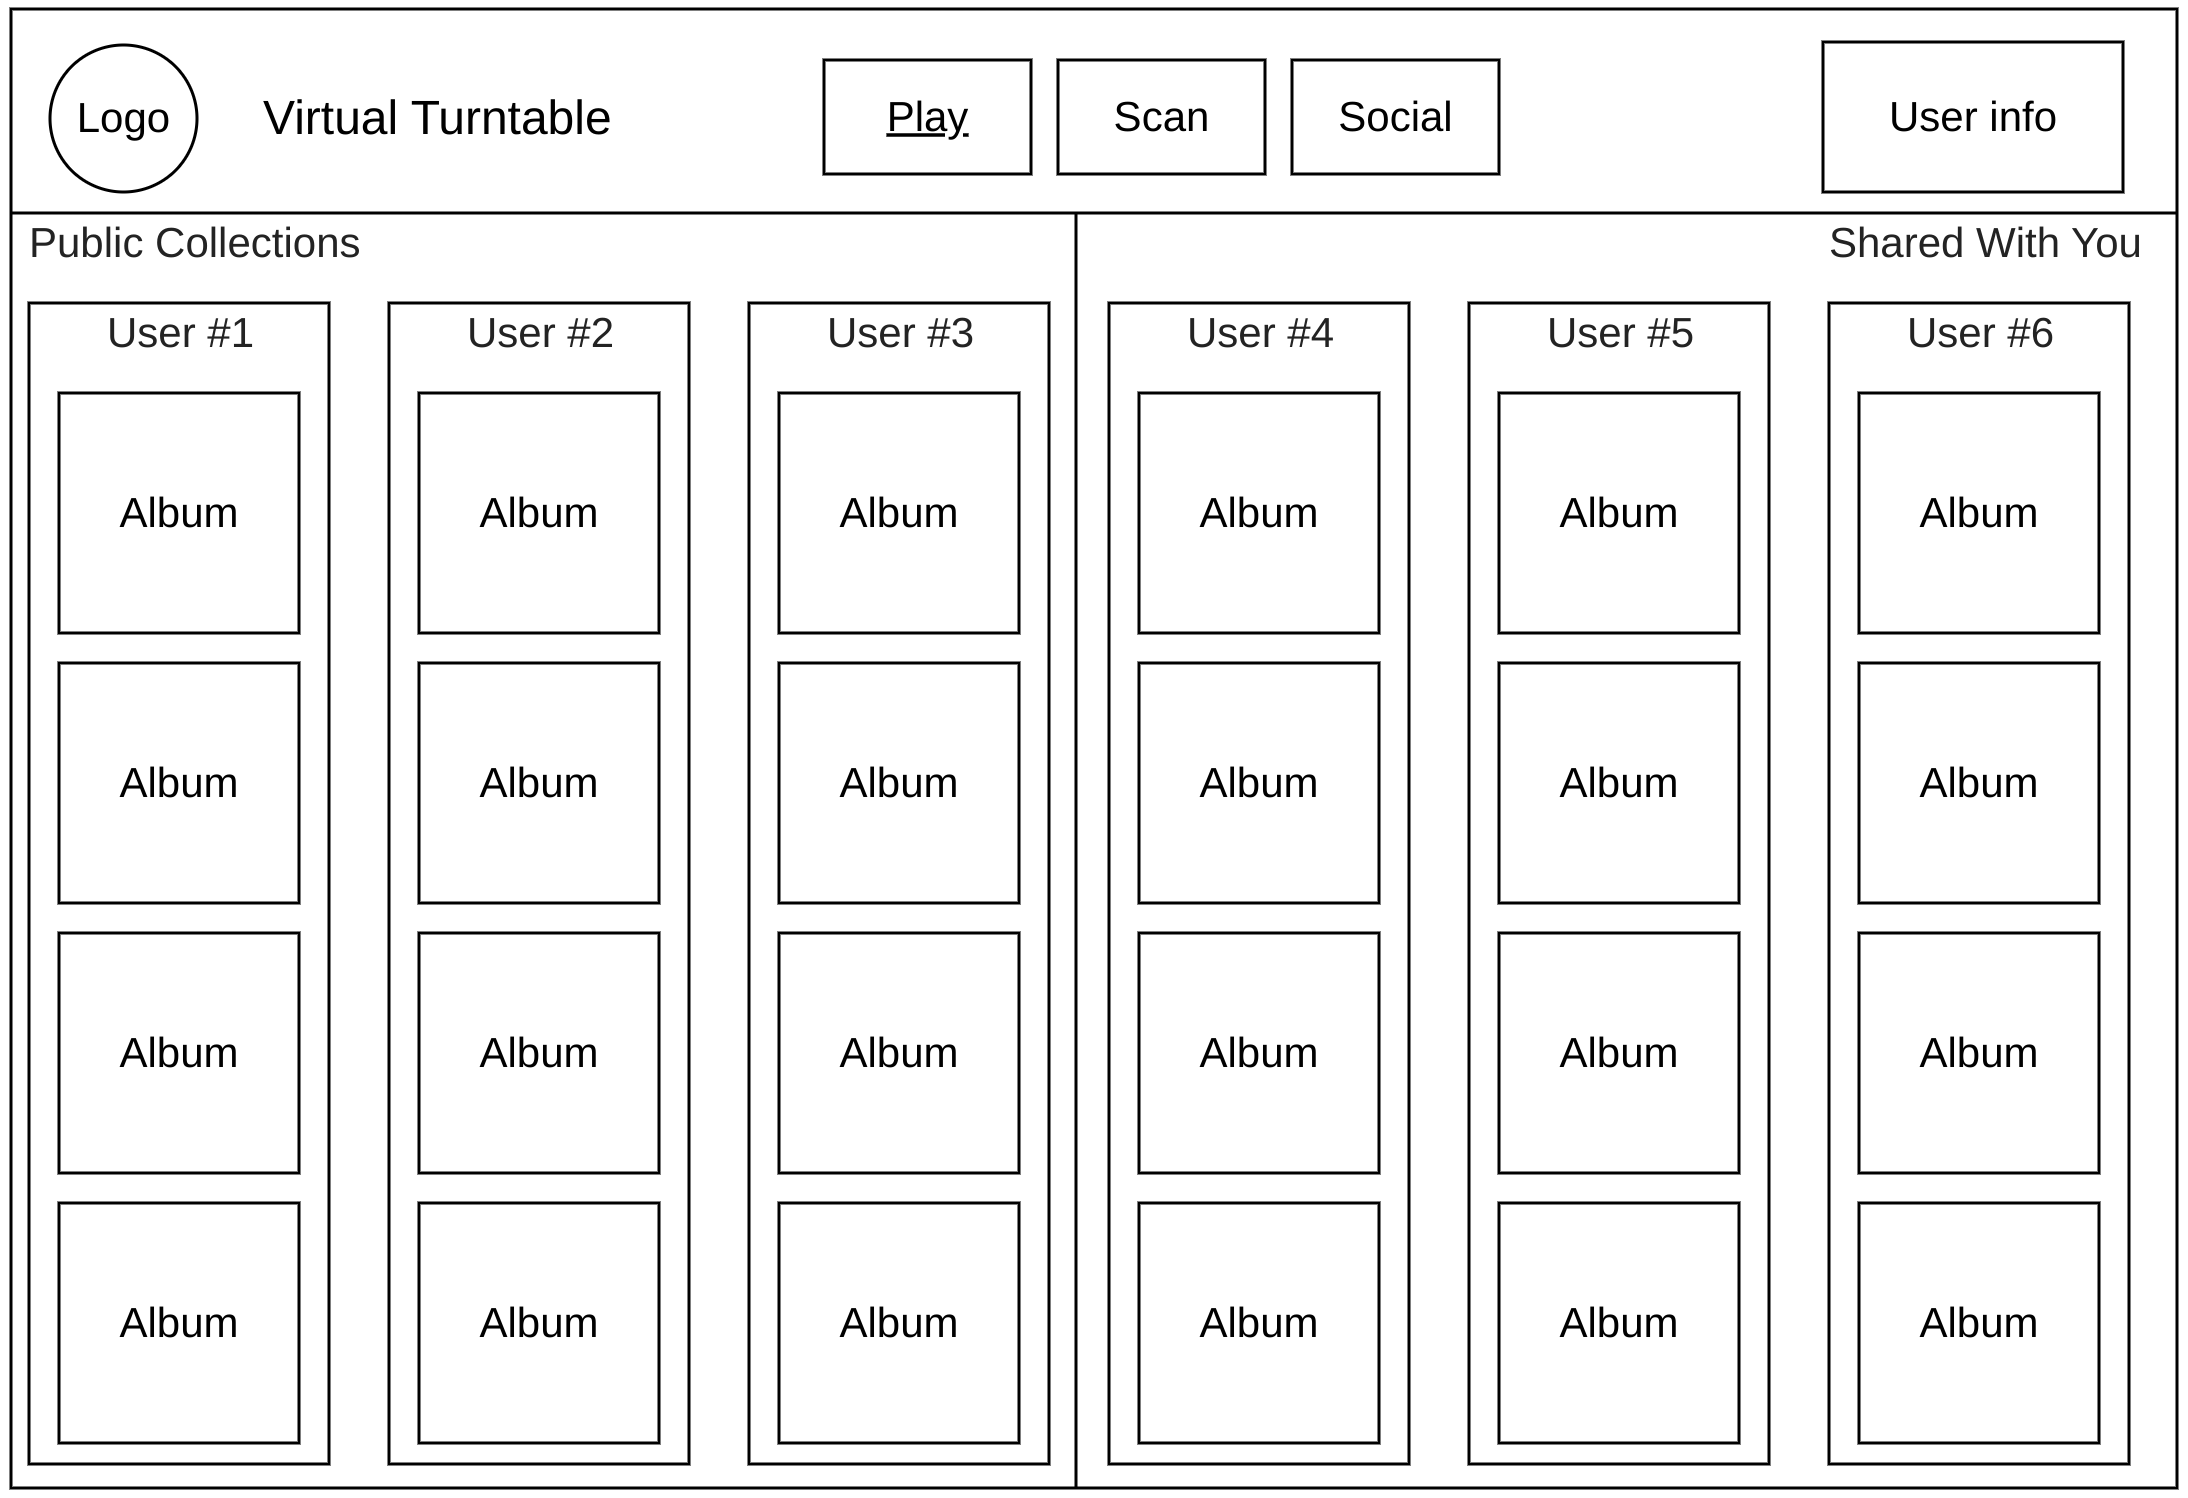
\includegraphics[width=0.6\linewidth]{figures/social_screen_mockup.png}
    \caption{The social screen wireframe mockup}
    \label{fig:social_screen_mockup}
\end{figure}



TODO: Add mockups and talk about why mockup the user interface and potentially stuff like fidelity

\section{Backend} \label{sec:backend-design}
\subsection{Microservices split} % Potentially change this
The split settled on is shown in Figure TODO:REF HERE. Including the BFF this involved splitting the backend into three pieces. This was chosen as

\subsubsection{BFF}
This service was the only service the frontend would ever talk to. It contained all endpoints that the frontend needed but did not implement much functionality other than calling other services.
\subsubsection{Image to Album}
This service would encompass all functionality regarding converting a representation of an album into a best guess of the album name. This could have been achieved in different ways: reverse image search, optical character recognition, or barcodes. Each of these could have been implemented as separate endpoints with the caller deciding which to use.
\subsubsection{User Data}
This service would encompass all operations related to non-volatile user data. This includes their own collections but also references to other collections that have been shared with them. To achieve this it had to be linked to a form of non-volatile store such as a database the design of which is detailed in Section~\ref{sec:database}.

TODO: Add details about choices about how the split into services was chosen. Reference literature talking about this stuff?

\subsection{Database} \label{sec:database}
The database for this project would store non-volatile user data mostly concerning

\subsubsection{SQL vs NoSQL}
TODO: Add discussion on why I didn't use NoSQL but mention the benefits that approach would have. Reference papers about NoSQL? (Especially in web development)
\subsubsection{UML Diagram}
TODO: Create and add UML diagram of the database and discussion of it
\subsubsection{DBMS Choice}


\section{Testing} \label{sec:test-design}
As part of the development life-cycle, validation tests must be made before development begins; this stops tests being made to fit the resulting product and so we can objectively see if it meets the initial criteria.


%Cite some references \cite{dyke1994, latex2012}
